\documentclass[11pt,a4paper]{article}
\usepackage[utf8x]{inputenc}
\usepackage[T1]{fontenc}
\usepackage{graphicx}
\usepackage[usenames, dvipsnames]{color}
\usepackage{fancyhdr}
\usepackage{datetime}
\setlength{\headheight}{15.2pt}
\pagestyle{fancy}
\fancyhf{}

\lhead{\textbf{\Large\color{MidnightBlue}Design and Modelling of Software Systems 
    \hfill Page: \thepage \\ ETFOS, 2011}}

\setlength{\parindent}{0cm}

\begin{document}
\large
Laboration Assignment No. 6 \\
Submission Date - \yyyymmdddate \today \\
Damir, Jelić, damir.jelic@etfos.hr \\
Marijan, Svalina, msvalina@etfos.hr
\\
\rule{\linewidth}{0.1mm}

\setcounter{section}{6}
\subsection{Phone lock class}
\begin{description}
    \item[Attributes:] \hfill
    \begin{itemize}
        \item is\_call
        \item lock\_code
        \item ap\_code
        \item reset\_time
        \item unlock\_time
    \end{itemize}
    \item[Methods:] \hfill
    \begin{itemize}
        \item lock()
        \item unlock()
        \item call()
        \item hangup()
        \item verificate\_phone\_code()
        \item verificate\_unlock\_code()
    \end{itemize}
\end{description}
\begin{description}
    \item[]
    The \emph{is\_call} attribute is a bool variable wich identifies if the user
    want's to unlock the door or call a apartment user.
    \item[]
    The \emph{lock\_code} and the \emph{ap\_code} are containers for valid 
    door unlock codes and apartment numbers.
    \item[]
    The \emph{reset\_time} and \emph{unlock\_time} store the values of the
    phone lock reset time (if no key is pressed) and how long the door stays
    unlocked.
    \item[]
    The \emph{lock()} and \emph{unlock()} methods control the door lock.
    \item[] 
    The \emph{call()} and \emph{hang\_up()} methods are used for establishing
    and terminating connections between the lock phone and the apartment phone.
    \item[]
    The \emph{verificate\_phone\_code} and \emph{verificate\_unlock\_code}
    methods check if the entered code is valid.

\end{description}

\newpage

\subsection{Phone lock state chart}
\begin{figure}[htb]
    \begin{center}
        \setlength\fboxsep{0pt}
        \fbox{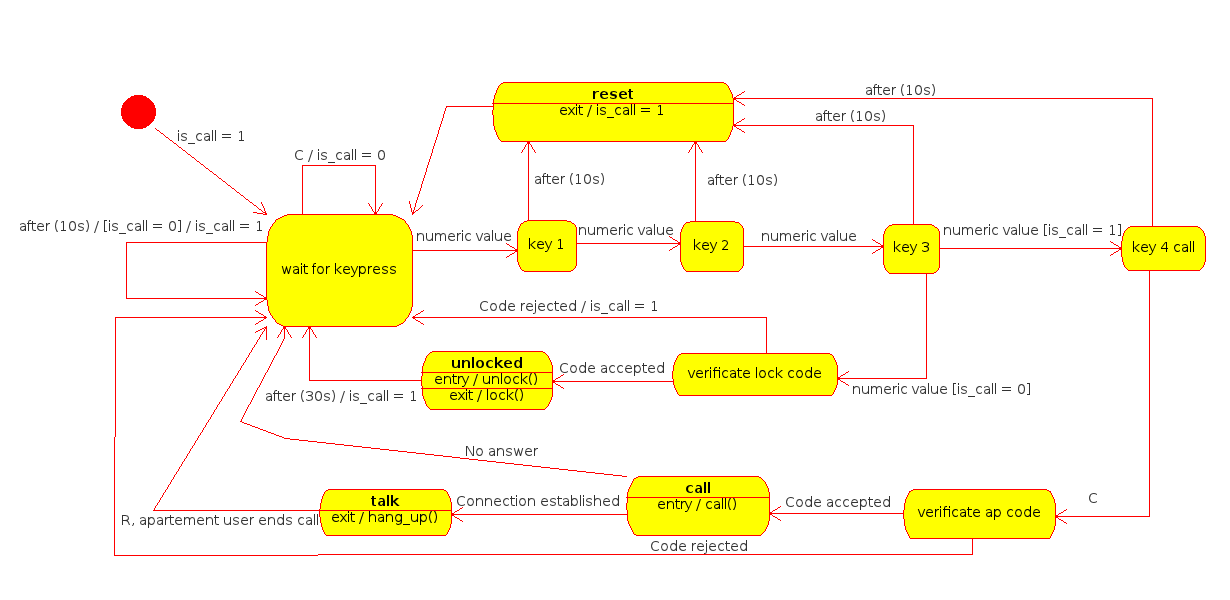
\includegraphics[scale=0.30]{state_diagram.png}}
        \caption{Phone lock state diagram}
        \label{fig:class_diag}
    \end{center}
\end{figure}
\begin{description}
    \item[]
    We start with the \emph{wait for keypress} state, if we press the \emph{C} key the system
    sets the \emph{is\_call} variable to 0 and stays in this state, 
    if we press a numeric key we go to the \emph{key 1} state.
    \item[]
    From the \emph{key 1} state we can proceed with a numeric key
    to the \emph{key 2} state from which also with a 
    numeric key procced to the \emph{key 3} state.
    \item[]
    In the \emph{key 3} state we can proceed with a numeric key but depending on the
    \emph{is\_call} attribute we go to different states. If the \emph{is\_call} is true
    we go to the \emph{key 4} state if it's false we go to the \emph{verificate lock code}
    state.
    \item[]
    From the \emph{key 4} state we can proceed with the \emph{C} key 
    to the \emph{verificate phone code} state.
    \item[]
    If we don't change states from the \emph{key 1-4} states in 10 seconds 
    we proceed to the \emph{reset} state which sets the \emph{is\_call} attribute
    to true and goes to the \emph{wait for keypress} state.
    \item[]
    The \emph{verificate lock code} state and the \emph{verificate phone code} state
    are used for code verification, if the code is rejected both go to the 
    \emph{wait for keypress} state.
    \item[]
    If the lock code is accepted we go to the \emph{unlocked} state wich unlocks the
    door upon entry and locks it upon exit, we go back to the \emph{wait for keypress}
    after 30 seconds and set the \emph{is\_call} attribute to 1.
    \item[]
    If the phone code is accepted we go to the \emph{call} state. The \emph{call} state
    tries to call the apartement user if the connection is established it proceeds to the
    \emph{talk} state if it fails to establish a connection it goes to the 
    \emph{wait for keypress} state.
    \item[]
    In the \emph{talk} state we can go back to the \emph{wait for keypress} state
    if the apartment user hangs up or if we press the \emph{R} key.
    \item[]
    A stop state isn't needed because the phone lock should always wait for a keypress.
\end{description}
\end{document}
